% Compile twice with pdfLaTeX from this directory.
% English slides, with speaker notes and timing in each frame.
% Define \presenternotes before input to produce a notes-only PDF.
\documentclass[aspectratio=1610,xcolor=dvipsnames,t]{beamer}
\usepackage{lmodern}
\usepackage{sansmath}
\usepackage{mathastext}
\usepackage{graphicx}
\usepackage{tikz}
\usetikzlibrary{decorations.pathreplacing}
\usepackage{beamerthemesplit}
% Reuse the theme stored in the sibling template directory.
\makeatletter
\def\input@path{{../模板/}}
\makeatother
\usetheme[compress]{Heidelberg}
\definecolor{unirot}{rgb}{0.5976525,0,0}
\usecolortheme[named=unirot]{structure}
\usepackage{amsmath,amssymb}
\newcommand{\toprule}{\hline}
\newcommand{\midrule}{\hline}
\newcommand{\bottomrule}{\hline}
\setbeamertemplate{headline}{}
\ifdefined\presenternotes
  \setbeameroption{show only notes}
\else
  \setbeameroption{hide notes}
\fi
\newcommand{\keyterm}[1]{\textcolor{unirot}{\textbf{#1}}}
% Keep existing backup content while suppressing per-slide source labels.
\newcommand{\papersource}[1]{}
\newcommand{\paperfig}[4][.50\textheight]{%
  \includegraphics[page=#2,viewport=#3,clip,width=#4,height=#1,keepaspectratio]{../2408.03314v1.pdf}}
\title[Test-Time Compute in LLMs]{Scaling LLM Test-Time Compute Optimally can be More Effective than Scaling Model Parameters}
\subtitle{Allocating inference compute under a fixed budget}
\author[Zhenbang Lyu]{Zhenbang Lyu}
\institute[Uni HD]{Heidelberg University\\Institute of Computer Science}
\date[]{Charlie Snell, Jaehoon Lee, Kelvin Xu, and Aviral Kumar\\2024, arXiv:2408.03314v1}

\begin{document}

\begin{frame}[plain]
  \titlepage
  \note{Time 0:00--0:30. The paper asks how to improve a fixed model by spending more computation when it answers a question. We will first examine how to allocate that computation, then compare it with training a larger model.}
\end{frame}

\begin{frame}{Can Language Models Benefit from More Thinking?}
  Humans often think for longer about difficult problems to reach better answers and improve their decisions.
  \par\medskip
  Extra thought gives us time to reconsider an initial answer and work through the reasoning more carefully.
  \par\medskip
  \keyterm{Can language models also improve their answers by using more computation at test time?}
  \par\medskip
  The paper studies how a trained model can use an additional inference budget on a challenging question.
  \note{Time 0:30--1:15. Follow the introduction's motivation. Humans tend to spend longer thinking about difficult problems to improve their decisions. Ask whether a trained language model can gain a similar ability. For a model, the resource we can allocate is additional computation during inference. The paper asks how effectively this resource can improve accuracy on a given prompt. Next make the available uses of that computation concrete.}
\end{frame}

\begin{frame}{How Do We Work through a Math Problem?}
  Suppose we want a better chance of finding the correct answer to a math problem.
  \par\medskip
  \begin{itemize}
    \item \textbf{Ask several people to solve it independently.} Collect their complete solutions, then compare the answers.
    \par\smallskip
    \item \textbf{Build on an existing attempt.} Read someone else's working and use it to develop an improved solution.
    \par\smallskip
    \item \textbf{Ask for feedback before we finished the question.} Show someone our unfinished reasoning before deciding how to continue.
  \end{itemize}
  \par\medskip
  \keyterm{A model can also try independently, revise earlier work, or use feedback during generation.}
  \note{Time 1:15--2:00. Start with several people independently solving the same problem. This motivates parallel sampling and best-of-N as the simplest baseline. Then introduce two ways to use existing work: revise an earlier attempt or obtain feedback before finishing. In the paper, parallel samples and revision history come from the model itself.}
\end{frame}

\begin{frame}{Two Directions for Using Extra Computation}
  \textbf{Baseline}\quad Generate $N$ independent solutions, then select an answer with a verifier: \keyterm{best-of-$N$}.
  \par\medskip
  The paper improves on this baseline in two directions.
  \par\smallskip
  \begin{itemize}
    \item \textbf{Change what the model generates.} Give it earlier answers and ask for a revised solution. \keyterm{Revisions} change its \textbf{proposal distribution}.
    \par\smallskip
    \item \textbf{Change how feedback guides generation.} Score partial solutions and choose which paths to develop. This is \keyterm{verifier-guided search}.
  \end{itemize}
  \par\medskip
  We first follow the verifier-guided search route from intermediate steps to a final answer.
  \note{Time 2:00--3:00. Map independent solvers to independent model samples. Best-of-N generates complete candidates and uses a verifier for final selection. The two improvements correspond to the proposer/verifier framework. Revisions condition on previous attempts. Search uses partial-solution scores. All share a finite budget. Focus on the verifier-guided route first and show the complete workflow before explaining its components.}
\end{frame}

\begin{frame}{PRM-Guided Search from Steps to an Answer}
  Score partial solutions and stop low-scoring branches before they become complete answers.
  \par\smallskip
  \begin{center}
  \resizebox{.96\textwidth}{!}{%
    \begin{tikzpicture}[x=1cm,y=.8cm,>=stealth,
      prefixnode/.style={draw=unirot,rounded corners=2pt,fill=unirot!4,minimum width=1.15cm,minimum height=.43cm,font=\small},
      stopped/.style={prefixnode,draw=black!25,fill=black!4,text=black!40},
      answernode/.style={draw=unirot,minimum width=.7cm,minimum height=.43cm,font=\small},
      flow/.style={->,line width=.7pt,draw=black!70},
      cutflow/.style={->,line width=.7pt,draw=black!30}]
      \node[font=\small] (q) at (0,-.25) {Question};
      \foreach \i/\h in {1/1.2,2/0,3/-1.2}{
        \node[prefixnode] (a\i) at (2.1,\h) {Step 1};
        \draw[flow] (q) -- (a\i);
      }
      \node[stopped] (a4) at (2.1,-2.3) {Step 1};
      \draw[cutflow] (q) -- (a4);
      \node[text=black!50,font=\large] at (2.95,-2.3) {$\times$};
      \foreach \i/\keep/\drop in {1/1.5/.85,2/.25/-.4,3/-1/-1.65}{
        \node[prefixnode] (b\i) at (4.9,\keep) {Step 2};
        \node[stopped] (c\i) at (4.9,\drop) {Step 2};
        \draw[flow] (a\i) -- (b\i);
        \draw[cutflow] (a\i) -- (c\i);
        \node[text=black!50,font=\large] at (5.75,\drop) {$\times$};
        \node (dots\i) at (6.7,\keep) {$\cdots$};
        \node[answernode] (y\i) at (8.1,\keep) {$Y_{\i}$};
        \draw[flow] (b\i) -- (dots\i);
        \draw[flow] (dots\i) -- (y\i);
      }
      \node[font=\small,text=unirot] at (4.4,2.2) {PRM scoring and pruning after each expansion};
      \node[draw=unirot,rounded corners=2pt,align=center,font=\small,minimum height=.72cm] (select) at (10.0,.25) {Answer\\selection};
      \node[font=\large,text=unirot] (final) at (12.0,.25) {$\hat{Y}$};
      \foreach \i in {1,2,3}{\draw[flow] (y\i) -- (select);}
      \draw[flow] (select) -- (final);
      \node[font=\small,text=black!60] at (7.6,-2.3) {$\times$ Pruned: no further generation};
    \end{tikzpicture}%
  }
  \end{center}
  \small
  Repeat until completion or the expansion limit. Three decisions remain:
  \begin{enumerate}
    \item Who scores the reasoning?
    \item How do we select the final answer?
    \item Which candidates should the search retain and expand?
  \end{enumerate}
  \note{Time 3:00--4:00. Follow the branching tree from the question. Gray nodes marked with a cross are pruned using PRM scores and receive no further generation. Retained Step 1 prefixes branch into different Step 2 candidates, which are scored and pruned again. Only surviving paths reach complete answers Y1, Y2, and Y3 for final selection. Standard best-of-N completes all independent candidates before selecting. Here partial-solution scores decide which branches receive later compute. The diagram is schematic and does not specify a fixed beam size. The next slides explain the scorer, final selection, and search rule.}
\end{frame}

\begin{frame}{Who Can Score the Reasoning?}
  Train a \keyterm{process reward model (PRM)} to predict the chance of finishing correctly from a given prefix.
  \par\smallskip
  \begin{center}
  \resizebox{.98\textwidth}{!}{%
    \begin{tikzpicture}[x=1cm,y=1cm,>=stealth,
      future/.style={draw=black!55,dashed,rounded corners=2pt,minimum height=.55cm,font=\small,align=center},
      rollout/.style={->,dashed,draw=black!55,line width=.7pt}]
      \node[draw=unirot,line width=.9pt,rounded corners=2pt,fill=unirot!4,
        align=center,minimum width=2.45cm,minimum height=1.1cm,font=\small] (prefix) at (1.3,0)
        {Question\\+ Steps $1,\ldots,t$};
      \node[font=\small,text=unirot] at (1.3,.95) {Current prefix};
      \node[font=\small] at (6.0,2.45) {Sample four continuations to complete answers};
      \foreach \i/\h in {1/1.8,2/.6,3/-.6,4/-1.8}{
        \node[future,minimum width=1.6cm] (next\i) at (4.6,\h) {Next steps};
        \node[future,minimum width=1.9cm] (answer\i) at (7.5,\h) {Final answer};
        \draw[rollout] (prefix.east) -- (next\i.west);
        \draw[rollout] (next\i.east) -- node[midway,fill=white,inner sep=2pt] {$\cdots$} (answer\i.west);
      }
      \foreach \i/\h in {1/1.8,2/.6,3/-.6}{
        \node[font=\Large,text=ForestGreen] at (8.85,\h) {$\checkmark$};
      }
      \node[font=\Large,text=unirot] at (8.85,-1.8) {$\times$};
      \draw[decorate,decoration={brace,amplitude=7pt},line width=.8pt,draw=black!65]
        (9.35,2.12) -- (9.35,-2.12);
      \node[align=center,font=\small] at (11.15,.95) {3 correct out of 4};
      \node[font=\Large,text=unirot] at (11.15,.1) {$\frac{3}{4}=0.75$};
      \node[align=center,font=\small,text=unirot] at (11.15,-.85) {Training target for\\the current prefix};
      \node[font=\small,text=black!60] at (6.3,-2.65) {Illustrative training rollouts. Dashed paths are possible futures.};
    \end{tikzpicture}%
  }
  \end{center}
  \small
  During search, the trained PRM \textbf{scores new prefixes directly}.
  \note{Time 4:00--5:15. Point to the solid box, which contains the question and the entire prefix through the current step. Hold that prefix fixed and independently sample four continuations with the base model, each all the way to a final answer. All future nodes and connecting paths are dashed. Check final correctness using ground truth during training. Three checks and one cross give an illustrative target of 3/4=0.75 for the current prefix. This estimates eventual success under the base model's sampling policy, not whether an isolated step is logically correct. Train the PRM to predict such targets from many prefixes. At search time the learned PRM directly scores a prefix without repeating these training rollouts. Four is an illustrative sample count, not the experiment's rollout count.}
\end{frame}

\begin{frame}{How Do We Select the Final Answer?}
  Use the PRM's \textbf{last-step score} for each complete solution, then sum scores for matching final answers.
  \par\medskip
  \begin{center}
  \begin{tabular}{lcc}
    \toprule
    Example candidate & Final answer & Last-step score\\
    \midrule
    $Y_1$ & $x=2$ & 0.60\\
    $Y_2$ & $x=2$ & 0.55\\
    $Y_3$ & $x=3$ & 0.90\\
    \bottomrule
  \end{tabular}
  \end{center}
  \[
    \operatorname{score}(x=2)=1.15,\qquad
    \operatorname{score}(x=3)=0.90
  \]
  \keyterm{Weighted best-of-$N$ selects $x=2$.}
  \par\smallskip
  Standard best-of-$N$ would pick the single highest-scoring candidate. Majority voting counts answers without weights.
  \note{Time 5:15--6:15. Answer the second workflow question using the three endpoints in the overview. The final-step PRM score sees the whole completed prefix. One aggregation turns step scores into a solution score; the other pools candidate scores by final answer. Candidate Y3 has the highest individual score, but x=2 has more total weighted support. A sum of 1.15 is not a probability. All numbers are illustrative. This is the final selection stage shared by the search methods. Next ask how the candidates themselves should be generated.}
\end{frame}

\begin{frame}{Which Candidates Should We Develop?}
  \begin{center}
    \paperfig[.53\textheight]{8}{61 493 551 710}{.98\textwidth}
  \end{center}
  \small
  \textbf{Best-of-$N$}\quad Generate independent complete solutions, then select.\\
  \textbf{Beam search}\quad Score prefixes, keep the top candidates, then expand.\\
  \textbf{Lookahead}\quad Temporarily continue $k$ steps before scoring a prefix.
  \par\smallskip
  Lookahead spends additional compute on its temporary continuations.
  \note{Time 6:15--7:45. Answer the third workflow question. Best-of-N waits until candidates are complete. Beam search allocates generation toward promising prefixes. Lookahead uses a temporary greedy continuation of up to k steps and scores its endpoint to evaluate the current prefix. The temporary steps help rank current prefixes. k=0 gives ordinary beam search. The paper estimates lookahead cost as N times k+1, so fair comparisons include that overhead. The detailed numerical example is in backup. Next compare these methods at matched compute budgets.}
\end{frame}


\begin{frame}{Beam Search Helps Most at Low Budgets}
  {\small PaLM 2-S* on MATH: 12,000 training questions and 500 test questions.}
  \par\medskip
  \begin{columns}[T,onlytextwidth]
    \begin{column}{.58\textwidth}
      \centering
      \paperfig[.61\textheight]{9}{61 539 309 708}{\linewidth}
    \end{column}
    \begin{column}{.39\textwidth}
      \small
      \textbf{Beam search is strongest at low budgets, but its advantage shrinks as compute increases.}
      \par\medskip
      At matched cost, extra lookahead usually gives less benefit.
    \end{column}
  \end{columns}
  \note{Time 7:45--9:00. Read Figure 3 left by comparing methods vertically at the same budget. Follow the beam-search curves from the low-budget region to higher budgets and compare with weighted best-of-N. Explain that lookahead's extra rollouts are charged to the budget. State both displayed conclusions. Then ask whether the aggregate trend hides different outcomes across question difficulty.}
\end{frame}

\begin{frame}{Difficulty Changes Which Search Strategy Wins}
  Each difficulty bin has four budgets, left to right: \textbf{4, 16, 64, 256}.
  \par\medskip
  \begin{columns}[T,onlytextwidth]
    \begin{column}{.52\textwidth}
      \centering
      \paperfig[.55\textheight]{9}{315 539 551 708}{\linewidth}
      \par\smallskip
      \small Read the top of each color. The bars overlap.
      \par\medskip
      \raggedright
      \small\textbf{Example, bin 2:} beam wins at budget 4. Best-of-$N$ wins at 256.
    \end{column}
    \begin{column}{.45\textwidth}
      \small
      \keyterm{Easy questions (bins 1--2)}
      \par\smallskip
      Beam search can win at small budgets, then stall or decline. Best-of-$N$ catches up.
      \par\medskip
      \keyterm{Medium difficulty (bins 3--4)}
      \par\smallskip
      Beam search consistently beats best-of-$N$ at the same budget.
      \par\medskip
      \keyterm{Hardest questions (bin 5)}
      \par\smallskip
      All three methods make little progress.
      \par\medskip
      \keyterm{Choose the search setting using both difficulty and budget.}
    \end{column}
  \end{columns}
  \note{Time 9:00--11:15. Figure 3 right and the paragraph Which problems does search improve? in Section 5.3 explicitly discuss these findings. Read the four positions within each difficulty bin as budgets 4, 16, 64, and 256. Blue is beam search, orange is weighted best-of-N, and green is majority voting. All bars start at zero and overlap, so compare the top of each color rather than adding the visible segments. In bin 2, compare blue and orange at budget 4, then at budget 256: the winner changes from beam search to best-of-N. In easy bins 1--2, beam search can improve initially and later stall or decline as the budget grows; the authors identify signs of over-optimization. This does not mean beam search always loses on easy questions or decreases at every budget increment. In bins 3--4, beam search consistently beats best-of-N at matched budgets. In bin 5, none makes meaningful progress. The authors suggest that stronger optimization may exploit imperfect PRM scores on easy questions, while on medium questions search helps guide a base model that rarely samples correct solutions. Treat this as their proposed explanation. The displayed conclusion motivates selecting the search setting by difficulty and budget in the next slide. Formal bin estimation remains in backup.}
\end{frame}

\begin{frame}{Less Compute Can Reach Similar Accuracy}
  \begin{columns}[T,onlytextwidth]
    \begin{column}{.58\textwidth}
      \centering
      \paperfig[.63\textheight]{10}{306 466 551 635}{\linewidth}
    \end{column}
    \begin{column}{.39\textwidth}
      \small
      \textbf{Choosing the search setting by difficulty can reach similar accuracy with less compute.}
      \par\medskip
      \textbf{Oracle at 16 generations:} almost the same accuracy as PRM best-of-$N$ weighted at 64.
      \par\medskip
      \textbf{Predicted at 16 generations:} also close to the same 64-generation baseline.
    \end{column}
  \end{columns}
  \par\smallskip
  {\small The compute used to estimate difficulty is not included.}
  \note{Time 11:15--12:00. Lead with the result: choosing the search setting by difficulty can reach similar accuracy with less compute. Find the green PRM best-of-N weighted curve at 64 generations, then compare the blue Oracle point at 16. The accuracy is almost the same, with the Oracle point slightly lower in the original figure. The orange Predicted point at 16 is also close to the green point at 64. Do not claim Oracle at 16 is higher, and do not state a multiplier. Briefly note that difficulty-estimation compute is excluded. Next move to revising earlier answers.}
\end{frame}

\begin{frame}{Revising Answers and Selecting the Output}
  A fine-tuned revision model uses earlier answer to write a new answer.
  \par\medskip
  \textbf{1\quad Generate}\quad Each call sees the question and up to four most recent answers.
  \begin{center}
  \resizebox{.97\textwidth}{!}{%
    \begin{tikzpicture}[x=1cm,y=1cm,>=stealth,
      revanswer/.style={minimum width=.86cm,minimum height=.58cm,font=\large},
      revflow/.style={->,line width=.75pt,draw=black!65}]
      \filldraw[fill=unirot!6,draw=unirot!65,rounded corners=3pt]
        (3.93,-.36) rectangle (8.97,.36);
      \node[revanswer,text=black!55] (a1) at (.6,0) {$A_1$};
      \node[revanswer,text=black!55] (a2) at (1.9,0) {$A_2$};
      \node[revanswer,text=black!55] (dots) at (3.2,0) {$\cdots$};
      \node[revanswer] (a60) at (4.5,0) {$A_{60}$};
      \node[revanswer] (a61) at (5.8,0) {$A_{61}$};
      \node[revanswer] (a62) at (7.1,0) {$A_{62}$};
      \node[revanswer] (a63) at (8.4,0) {$A_{63}$};
      \node[revanswer,draw=unirot,rounded corners=3pt,text=unirot] (a64) at (10.7,0) {$A_{64}$};
      \draw[revflow] (a1) -- (a2);
      \draw[revflow] (a2) -- (dots);
      \draw[revflow] (dots) -- (a60);
      \draw[revflow] (a60) -- (a61);
      \draw[revflow] (a61) -- (a62);
      \draw[revflow] (a62) -- (a63);
      \draw[revflow] (a63) -- (a64);
      \node[font=\small,text=black!55] at (1.9,.88) {Earlier answers};
      \node[font=\small,text=unirot] at (6.45,.88)
        {Input for $A_{64}$: $q+A_{60}+A_{61}+A_{62}+A_{63}$};
      \node[font=\small,text=unirot] at (6.45,-.75) {The four-answer context window};
      \node[font=\small,text=black!60] at (10.7,-.75) {New answer};
    \end{tikzpicture}%
  }
  \end{center}
  \textbf{2\quad Select}\quad Use ORM weighted selection within each chain, then across chains.
  \begin{center}
  \resizebox{.96\textwidth}{!}{%
    \begin{tikzpicture}[x=1cm,y=1cm,>=stealth,
      pickflow/.style={->,line width=.75pt,draw=black!65}]
      \node[font=\small,text=black!60] at (1.9,1.0) {All candidates};
      \node[font=\small,text=black!60] at (5.8,1.0) {One answer per chain};
      \node[font=\large] (pa) at (1.9,.4) {$\{A_1,\ldots,A_{64}\}$};
      \node[font=\large] (pb) at (1.9,-.4) {$\{B_1,\ldots,B_{64}\}$};
      \node[font=\large] (ya) at (5.8,.4) {$\hat A$};
      \node[font=\large] (yb) at (5.8,-.4) {$\hat B$};
      \node[draw=unirot,rounded corners=3pt,font=\small,align=center,
        minimum width=1.8cm,minimum height=.85cm] (across) at (8.5,0) {ORM weighted\\across chains};
      \node[font=\Large,text=unirot] (y) at (10.7,0) {$\hat y$};
      \draw[pickflow] (pa) -- (ya);
      \draw[pickflow] (pb) -- (yb);
      \draw[pickflow] (ya) -- (across);
      \draw[pickflow] (yb) -- (across);
      \draw[pickflow] (across) -- (y);
    \end{tikzpicture}%
  }
  \end{center}
  {\small A later revision can undo a correct answer, so select from the saved history.}
  \note{Time 12:00--13:15. A revision model uses previous complete answers. The first call sees only the question. At round 64 it sees the question and answers 60 through 63; older answers remain saved. The lower diagram illustrates the revision ORM's hierarchical selection with multiple chains. Within each chain, sum ORM scores by final answer, choose the winning answer value, and retain its highest-scoring solution as the chain representative. Then apply best-of-N weighted again to the representatives across chains. Two chains of length 64 give 128 candidates before selection. This hierarchy is for the ORM, not majority voting. Majority voting pools all answers from all chains once, as specified in Appendix I. The revision experiments use a separately trained ORM, as specified in Appendix J. A later revision can undo a correct answer. The next figure compares fixed-round answer quality with selected-answer accuracy; Figure 7 then studies different numbers and lengths of chains.}
\end{frame}

\begin{frame}{Revision Quality and Final Answer Accuracy}
  \begin{center}
    \paperfig[.58\textheight]{12}{61 539 551 715}{.98\textwidth}
  \end{center}
  \small
  \begin{columns}[T,onlytextwidth]
    \begin{column}{.48\textwidth}
      \textbf{Four chains per question.}
      \par\smallskip
      Average correctness at the same round.
      \par\smallskip
      No voting or ORM selection.
    \end{column}
    \begin{column}{.48\textwidth}
      \textbf{Sequential:} $N$ answers in one chain.
      \par\smallskip
      \textbf{Parallel:} $N$ independent answers.
      \par\smallskip
      Majority or ORM-weighted voting.
    \end{column}
  \end{columns}
  \par\medskip
  \begin{columns}[T,onlytextwidth]
    \begin{column}{.48\textwidth}
      \centering
      \keyterm{Most improvement happens in early rounds.}
    \end{column}
    \begin{column}{.48\textwidth}
      \centering
      \keyterm{Sequential is slightly better with either selector.}
    \end{column}
  \end{columns}
  \note{Time 13:15--15:00. Verified against Figure 6 and Section 6.1 on paper pages 11--12, and Appendix I--J on page 26. Left: for each question, generate four revision trajectories of length 64. At round t, check only the t-th complete answer from each trajectory, average correctness over the four trajectories, and then over all 500 test questions. There is no majority vote or ORM selection within or across trajectories for this plotted pass@1 metric. Most improvement happens in early rounds. Right: compare N complete answers in one sequential chain against N independent initial answers from the same revision model. For sequential majority, count final-answer values among the N answers in that one chain. For sequential best-of-N weighted, sum ORM scores by final-answer value among those same N answers and choose the greatest total. Apply these same two selection rules to the N independent answers in the parallel case. These two generation styles and two selectors give the four curves. Evaluate one selected answer per question. This comparison does not combine several multi-answer revision chains using hierarchical selection. Figure 7 on the next slide studies those mixed configurations. Sequential is slightly better with either selector. Appendix I specifies the hierarchical ORM rule for the mixed case and a single pooled vote for majority. Appendix J identifies the separate revision ORM.}
\end{frame}

\begin{frame}{The Best Mix Depends on Difficulty and Budget}
  \small
  \textbf{Both figures:} ORM weighted selection within each chain, then across chains.
  \begin{center}
    \paperfig[.42\textheight]{13}{61 539 551 708}{.98\textwidth}
  \end{center}
  \begin{columns}[T,onlytextwidth]
    \begin{column}{.48\textwidth}
      \textbf{Left: each line fixes the total budget.}
      \par\smallskip
      \keyterm{At high budgets, a mix can beat both extremes.}
    \end{column}
    \begin{column}{.48\textwidth}
      \textbf{Right: 128 answers, grouped by difficulty.}
      \par\smallskip
      \keyterm{Easy questions favor longer chains; harder ones often need more starts.}
    \end{column}
  \end{columns}
  \par\smallskip
  \begin{center}
  \resizebox{.96\textwidth}{!}{%
    \begin{tikzpicture}[x=1cm,y=1cm,>=stealth,
      chainstage/.style={draw=unirot,rounded corners=2pt,align=center,font=\small,minimum height=.65cm},
      chainarrow/.style={->,line width=.8pt,draw=black!65}]
      \node[chainstage,minimum width=3.0cm] (all) at (1.6,0) {128 answers\\8 chains $\times$ 16};
      \node[chainstage,minimum width=2.8cm] (representatives) at (7.0,0) {8 representative\\solutions};
      \node[chainstage,minimum width=2.0cm] (final) at (12.2,0) {1 final\\answer};
      \draw[chainarrow] (all) -- node[above,font=\scriptsize] {within-chain ORM} (representatives);
      \draw[chainarrow] (representatives) -- node[above,font=\scriptsize] {across-chain ORM} (final);
    \end{tikzpicture}%
  }
  \end{center}
  \note{Time 15:00--16:45. Figure 7 uses ORM-based selection in both figures. First explain the shared example: 128 generations can be eight independent revision chains with sixteen complete answers in each. The sequential-to-parallel ratio is chain length divided by chain count, so this example has ratio sixteen divided by eight, or two. Within each chain, use best-of-N weighted to choose an answer value and retain its highest-scoring solution. This produces eight representatives. Apply best-of-N weighted again across those representatives to get one final answer. Measure the final selected answer's correctness, then average over questions. These are the selection rules in Appendix I, using the revision ORM from Appendix J. The left figure varies the ratio at each fixed total budget; our example is one setting on the budget-128 line. The right figure fixes the total budget at 128 and compares ratios within each difficulty group, using the same selection procedure. With only one chain, cross-chain selection is trivial; with one answer per chain, within-chain selection is trivial. At high budgets a mix can outperform the pure extremes. Easy questions favor longer chains; harder questions often need more independent starts. Majority voting is not used in Figure 7.}
\end{frame}

\begin{frame}{Adaptive Revisions Use the Generation Budget More Efficiently}
  \begin{columns}[T,onlytextwidth]
    \begin{column}{.58\textwidth}
      \centering
      \paperfig[.63\textheight]{13}{306 186 551 357}{\linewidth}
    \end{column}
    \begin{column}{.39\textwidth}
      \small
      \textbf{Adaptive revisions keep improving after parallel sampling begins to plateau.}
      \par\medskip
      \keyterm{64 candidates can beat parallel best-of-$N$ with 256 candidates.}
      \par\medskip
      Both oracle and predicted difficulty improve the allocation.
    \end{column}
  \end{columns}
  \par\smallskip
  {\small The reported saving excludes difficulty-estimation cost.}
  \note{Time 16:45--17:45. Figure 8 compares adaptive mixtures with pure parallel sampling. Solid lines use the revision ORM with best-of-N weighted within each chain and then across chain representatives. Dashed lines use majority voting over all candidate answers from all chains at once, not hierarchical voting. Colors distinguish oracle, predicted, and parallel. Compare within a selection rule. Read across budgets for the 64-versus-256 example. State the displayed conclusions and the excluded difficulty cost. Next compare extra inference with larger model size at equal total FLOPs.}
\end{frame}

\begin{frame}{Comparing Two Uses of the Same Compute}
  Compare the same total FLOPs, counting \textbf{pretraining and inference}.
  \par\bigskip
  \begin{columns}[T,onlytextwidth]
    \begin{column}{.48\textwidth}
      \keyterm{Train a larger model}
      \par\smallskip
      About 14$\times$ as many parameters.
      \par\smallskip
      Generate one greedy answer per question.
    \end{column}
    \begin{column}{.48\textwidth}
      \keyterm{Use more inference}
      \par\smallskip
      Keep the smaller model.
      \par\smallskip
      Spend extra compute on search or revisions.
    \end{column}
  \end{columns}
  \par\bigskip
  The smaller model can use its pretraining savings for extra inference.
  \par\medskip
  \keyterm{Which option gives higher accuracy at the same total cost?}
  \note{Time 17:45--19:00. Compare the two options in Section 7, paper pages 14--15. Count pretraining plus inference FLOPs for the same planned workload. The larger model has about 14 times as many parameters, uses the same pretraining token count, and generates greedy answers. The smaller model can use the pretraining savings for additional search or revisions. Ask which option gives higher accuracy at the same total cost, then move to Figure 9. Details of the token-workload ratio, numerical budget matching, and algebra are in backup slide 25.}
\end{frame}

\begin{frame}{Extra Inference Can Beat a Larger Model in Some Settings}
  \begin{center}
    \paperfig[.47\textheight]{15}{64 526 549 715}{.98\textwidth}
  \end{center}
  \small
  \begin{itemize}
    \item Extra inference often wins on easy or medium questions, especially when expected inference use is low.
    \item A larger model is often better on very hard questions or when expected inference use is high.
  \end{itemize}
  \par\smallskip
  \keyterm{The comparison depends on both difficulty and the expected inference workload.}
  \note{Time 19:00--21:30. Read Figure 9. Apply the equal-total-cost comparison introduced on the previous slide. Each vertical comparison line represents a different planned inference workload and its matched budget. Numerical workload ratios and their derivation remain in backup slide 25. Curves are adaptive inference with the small model, stars are greedy answers from the model with about 14 times more parameters. Match color and the workload's vertical line. A curve higher than the star favors additional inference. The same star height repeats at different matched budgets. Purple easy questions and blue hardest questions show different patterns. State both displayed conditional findings. Figure 9 uses oracle difficulty bins. Move directly to the conclusions, bringing together the search results, revision results, and the equal-cost comparison.}
\end{frame}

\begin{frame}{Conclusions}
  \begin{itemize}
    \item \textbf{PRM search.} Beam search works better on harder questions and at low budgets. Best-of-$N$ often wins on easier questions or at high budgets.
    \par\smallskip
    \item \textbf{Revisions.} Easy questions favor longer chains. Harder questions often need a mix of sequential revisions and independent starts.
    \par\smallskip
    \item \textbf{Allocation by difficulty and budget.} Search nearly matches best-of-$N$ with \keyterm{\mbox{16 vs.\ 64}} generations. Revisions can beat it with \keyterm{\mbox{64 vs.\ 256}}.
    \par\smallskip
    \item \textbf{Training versus inference.} At equal total FLOPs, extra inference can beat a model with \keyterm{$\sim$14$\times$ more parameters}. Very hard questions or a high inference workload often favor pretraining.
  \end{itemize}
  \par\medskip
  {\footnotesize Generation budgets exclude difficulty-estimation compute.}
  \note{Time 21:30--23:30. Summarize all three experimental parts, using the takeaways in Section 5.3 (paper page 10), Section 6.2 (page 14), Section 7 (page 15), and the opening summary of Section 8 (pages 15--16). PRM search: the best method depends on both budget and model-relative question difficulty. Beam search is useful at low budgets and on difficulty bins 3--4, while best-of-N is often preferable on easier questions or at larger budgets. This is not a claim that beam search solves the hardest bin. Revisions: simple questions favor long sequential chains, while harder questions often need several independent starts as well. Adaptive allocation is the common principle. Figure 4's 16-versus-64 comparison is nearly matching, not an exact accuracy win. Figure 8's 64-versus-256 comparison can favor revisions. These generation budgets exclude the difficulty-estimation cost. Finally, Figure 9 compares total pretraining plus inference FLOPs, with fixed pretraining token counts. A small model using extra inference can beat one with about 14 times more parameters when the questions are within reach or the inference workload is low. The hardest questions and high inference workloads often favor additional pretraining. The paper therefore does not find pretraining and test-time compute interchangeable for all settings.}
\end{frame}

\begin{frame}{Questions}
  \vfill
  \begin{center}
    {\Huge\color{unirot}\textbf{Thank you}}\\[.4cm]
    {\Large Questions and Discussion}
  \end{center}
  \vfill
  \note{Questions follow the main talk. Backup slides cover revision training, revision failures, beam search, difficulty estimation, and the full cost equations.}
\end{frame}

\appendix

\begin{frame}{Backup: Constructing Revision Training Data}
  \begin{columns}[T,onlytextwidth]
    \begin{column}{.43\textwidth}
      \textbf{Build a training pair}
      \par\medskip
      \begin{itemize}
        \item Sample 64 independent answers to one question.
        \item Choose a correct answer as the target.
        \item Add 0--4 related incorrect answers as context.
        \item Prefer close pairs using character edit distance.
      \end{itemize}
    \end{column}
    \begin{column}{.53\textwidth}
      \textbf{An illustrative pair}
      \par\medskip
      Question: solve $2x+3=7$.
      \par\medskip
      \textbf{Incorrect reference}
      \[
        2x=4,\qquad x=4
      \]
      \textbf{Correct target}
      \[
        2x=4,\qquad \textcolor{unirot}{x=2}
      \]
      The target keeps the valid setup and fixes the final calculation.
    \end{column}
  \end{columns}
  \par\medskip
  Fine-tune on \textbf{question + incorrect references} as input, with the \textbf{correct solution} as the target.
  \note{Optional backup. The example is illustrative. In the experiment, 64 complete answers per question are sampled independently at a higher temperature and assembled into synthetic revision trajectories afterward. The number of incorrect reference answers is sampled uniformly from zero through four. Character edit distance prioritizes related incorrect and correct solutions. In the example the setup is shared and the correct target repairs the final calculation. This encourages using earlier work. Edit distance is a heuristic for relatedness and is used to build training pairs. At inference, the window is the most recent four answers in chronological order.}
\end{frame}

\begin{frame}{Backup: Why the Last Revision Can Be Wrong}
  \begin{tabular}{@{}ll@{}}
    \textbf{Training history} & Incorrect references, followed by a correct target.\\[1mm]
    \textbf{Inference history} & Generated references can already be correct.
  \end{tabular}
  \par\medskip
  A possible revision chain, illustrated on $2x+3=7$:
  \begin{center}
    \begin{tikzpicture}[x=1cm,y=1cm,>=stealth,
      toyanswer/.style={draw=black!35,rounded corners=3pt,align=center,
        minimum width=2.4cm,minimum height=1.0cm,font=\normalsize}]
      \node[toyanswer] (a) at (0,0) {$A_1$: $x=4$\\Incorrect};
      \node[toyanswer,draw=ForestGreen,text=ForestGreen] (b) at (4.0,0) {$A_2$: $x=2$\\Correct};
      \node[toyanswer] (c) at (8.0,0) {$A_3$: $x=5$\\Incorrect};
      \draw[->,line width=.8pt,draw=black!60] (a) -- node[above,font=\small] {revise} (b);
      \draw[->,line width=.8pt,draw=black!60] (b) -- node[above,font=\small] {revise} (c);
    \end{tikzpicture}
  \end{center}
  \par\medskip
  {\Large\color{unirot}\textbf{About 38\%}} of correct answers became incorrect under the authors' naive revision approach.
  \par\medskip
  Selecting from the history gives the system a chance to recover an earlier correct answer.
  \note{Optional backup. The three-answer chain is a schematic example, not measured outputs. The reported 38 percent concerns correct answers converted to incorrect ones under naive revision, not 38 percent of all generated answers. This is consistent with a distribution shift: training references were incorrect, while generated inference history can already contain correct answers. Selecting from history can recover a correct answer, but neither verifier selection nor majority voting guarantees correctness. Figure 6 right compares sequential and parallel generation after selection, rather than directly comparing last-answer submission with selection.}
\end{frame}



\begin{frame}{Backup: A Complete Beam-Search Example}
  Suppose each round maintains $N=6$ candidates and each retained prefix gets $M=2$ continuations.
  \par\medskip
  \begin{enumerate}
    \item Generate 6 possible first steps and score their prefixes with the PRM.
    \item Keep the top $N/M=3$ prefixes.
    \item Extend each twice, giving $3\times2=6$ candidates for the next round.
    \item Repeat scoring and expansion until completion or 40 rounds.
    \item Apply weighted best-of-$N$ to the final candidates and return one answer.
  \end{enumerate}
  \par\medskip
  \keyterm{The base model proposes, the PRM scores, search allocates effort, and final selection chooses the output.}
  \note{Optional backup. Recap the complete process after explaining the three components. Pruning happens across all candidate prefixes, so two descendants of one prefix can both survive. N is the candidate pool and M is the number of continuations per retained prefix in this implementation. The general workflow drawing omitted these algorithm-specific settings. Forty is the paper's maximum expansion count. Use this example if a question calls for the detailed expansion and pruning procedure.}
\end{frame}


\begin{frame}{Backup: Difficulty Estimation and Policy Selection}
  Test this idea with \textbf{PaLM 2-S* (Codey)} on \textbf{MATH}: 12,000 training questions and 500 test questions.
  \par\medskip
  \begin{enumerate}
    \item Estimate difficulty from 2,048 independent samples per question.
    \item Sort questions into five equal-frequency bins, from easy to hard.
    \item For each bin and budget, select a setting on one fold and evaluate on the other. Swap folds and average.
  \end{enumerate}
  \par\smallskip
  \begin{tabular}{@{}ll@{}}
    \textbf{Oracle bins} & Rank by actual correctness rate.\\
    \textbf{Predicted bins} & Rank by the verifier's mean final-answer score.
  \end{tabular}
  \par\medskip
  \keyterm{Reported budgets exclude difficulty-estimation cost.}
  \note{Optional backup. With a trained verifier available, return to choosing an allocation by difficulty. Briefly introduce PaLM 2-S* and MATH, with 12,000 training and 500 test questions. Use actual correctness or mean verifier scores to construct two separate five-bin partitions. The latter avoids needing ground-truth answers when scoring difficulty. Choose settings on one fold and evaluate on the other, then swap and average. Difficulty-estimation cost is excluded. We now have a scorer and a selection rule; next explain how its scores determine a final answer.}
\end{frame}




\begin{frame}{Backup: Pretraining and Inference at Equal Total FLOPs}
  Extra inference improves the small model. How does it compare with training a larger model?
  \par\smallskip
  Hold training tokens fixed and increase parameters by a factor $M$.
  \[
    X\approx6PD_{\mathrm{pretrain}},\qquad
    Y\approx2PD_{\mathrm{inference}}
  \]
  $P$ is the parameter count. $D_{\mathrm{inference}}$ is the total inference token workload.
  \par\medskip
  \[
    \underbrace{X+aY}_{\text{small model, extra inference}}
    =\underbrace{M(X+Y)}_{\text{large model, greedy decoding}}
  \]
  \par\medskip
  The larger model costs more both to train and to run. The small model can spend its training savings on inference.
  \note{Optional backup. Section 7, paper page 14. Move from choosing inference strategies to choosing where to spend the total compute budget. P denotes parameter count, distinct from earlier candidate count N. X and Y are the small model's baseline training and inference costs. The larger model costs M times as much for both, with training tokens fixed. The small model can use the training savings for more inference. We next calculate how much extra inference that buys.}
\end{frame}

\begin{frame}{Backup: Using R to Compare Total Compute}
  \small
  $R$ is baseline inference tokens divided by pretraining tokens:
  \[
    R=\frac{D_{\mathrm{inference}}}{D_{\mathrm{pretrain}}}.
  \]
  From $X+aY=M(X+Y)$, the small model's inference multiplier is
  \[
    \begin{aligned}
      a &= M+(M-1)\frac{X}{Y}
       = M+(M-1)\frac{6P D_{\mathrm{pretrain}}}{2P D_{\mathrm{inference}}}\\
        &= M+3(M-1)\frac{D_{\mathrm{pretrain}}}{D_{\mathrm{inference}}}
         = M+\frac{3(M-1)}{R}.
    \end{aligned}
  \]
  \begin{center}
  \renewcommand{\arraystretch}{1.15}
  \begin{tabular}{@{}lccc@{}}
    \textbf{$R$} & 22 & 0.79 & 0.16\\
    \textbf{Small-model inference budget} & $\sim16\times$ & $\sim64\times$ & $\sim256\times$
  \end{tabular}
  \end{center}
  {\footnotesize Approximate multipliers for $M\approx14$, relative to baseline inference.}
  \par\smallskip
  \keyterm{These budgets set the stars' horizontal positions in Figure 9.}
  \note{Optional backup. Section 7, paper pages 14--15. This slide combines the full derivation with the budget examples moved out of main slide 16. R is the dimensionless ratio of total baseline inference tokens to pretraining tokens. Fix this baseline workload before adding extra inference; R is not itself a FLOPs cost or an inference multiplier. Solve X+aY=M(X+Y) for a, substitute the FLOPs approximations, cancel the parameter count, and use Dpretrain/Dinference=1/R. For M approximately 14, the paper's rounded R values 22, 0.79, and 0.16 correspond approximately to multipliers 16, 64, and 256. These budgets identify equal-total-cost positions on the x-axis of Figure 9. The large model still uses greedy decoding, so each color's star stays at the same accuracy across positions. At a fixed R, giving the small model more compute than the matched budget increases its total cost above the large model's.}
\end{frame}

\end{document}
